\begin{enumerate}[itemsep = 5mm]
		\item \textbf{Affirmation 1 : Fausse.}

		On construit rapidement le tableau de signes de $f$ :
		\begin{center}
		\begin{tikzpicture}
			\tkzTabInit[lgt = 3]
				{$x$/0.85,signe de $x+1$/.85,signe de $x-3$/0.85,signe de $x-5$/0.85,signe de $f(x)$/0.85}
				{$-\infty$,$-1$,$3$,$5$,$+\infty$}
				\tkzTabLine{,-,z,+,t,+,t,+, }
				\tkzTabLine{,-,t,-,z,+,t,+, }
				\tkzTabLine{,-,t,-,t,-,z,+, }
				\tkzTabLine{,-,z,+,z,-,z,+, }
		\end{tikzpicture}
		\end{center}
		Donc $f$ est positive sur \mbox{$[-1;3]$}.

		\item \begin{enumerate}
			\item \textbf{Affirmation 2 : Vraie.}

			Pour tout $x$ réel, on a :\quad \mbox{$h'(x) = -6x+12$},

			donc \quad \mbox{$h'(1) = 6$} : \quad la pente  de la tangente est $6$.

			Donc son équation est du type \quad \mbox{$y = 6x+b$}, \quad où $b$ désigne l'ordonnée à l'origine.

			Comme \quad \mbox{$h(1) = 5$},\quad la tangente doit passer par ce point. On écrit \mbox{$6\times1+b = 5$}, donc \mbox{$b = -1$}.

			L'équation de la tangente en $1$ est effectivement \mbox{$y = 6x-1$}.

			\emph{Remarque :} On peut aussi utiliser directement la formule qui donne l'équation de la tangente : \quad $y = h'(a)(x - a) + h(a)$

			Ici, on veut la tangente au point d'abscisse 1, donc $a = 1$.

			$y = h'(1)(x - 1) + h(1)$.

			En remplaçant les valeurs connues :\quad $y = 6(x - 1) + 5$

			On simplifie : \quad $y = 6x - 6 + 5$\quad soit \quad $y = 6x - 1$.

			\item \textbf{Affirmation 3 : Fausse.}

			Sur $[2 ; +\infty[$, on a : \quad $\begin{aligned}[t]
				x \geqslant 2
				&\implies -6x \leqslant -12 \quad \text{car } -6 < 0\\
				&\implies -6x + 12 \leqslant 0
			\end{aligned}$

			$h'$ change de signe en 2 : la dérivée de $h$ est négative sur \mbox{$[2;+\infty[$}, $h$ est donc décroissante sur cet intervalle (elle est même strictement décroissante sur l'intervalle, car la dérivée ne s'annule que pour $x = 2$), c'est la stricte décroissance qui garantit que la fonction n'est pas croissante.

			\emph{Remarque :} On peut aussi ici justifier cela sans la fonction dérivée : on sait que la fonction $h$ a un coefficient dominant strictement négatif (c'est $-3$), et donc, par propriété du cours, on sait que la fonction sera d'abord croissante, puis décroissante, avec un changement de variation pour $x = \dfrac{-b}{2a} = \dfrac{-12}{2\times (-3)} = 2$.

			Sans même savoir où la fonction va changer de sens, on peut dire que de toutes façons, sur un intervalle non majoré, la fonction ne peut pas être croissante sur l'intervalle, à cause du coefficient dominant négatif.
		\end{enumerate}

		\item \textbf{Affirmation 4 : Vraie.}

		Puisque $2$ est une racine de $g$ et que l'axe de symétrie est la droite $x = \np{2.5}$, cela signifie que l'autre racine de $g$ est $3$ : en effet les deux racines sont à la même distance de l'axe de symétrie.


		Donc \quad \mbox{$g(x) = (x-2)(x-3)$} \quad et \quad $g(0) = (-2)\times(-3) = 6$.

	\end{enumerate}
